\documentclass{ieeeaccess}

\usepackage{cite}
\usepackage{amsmath,amssymb,amsfonts}
\usepackage{algorithmic}
\usepackage{graphicx}
\usepackage{textcomp}
\usepackage{array}

\graphicspath{{figures/}{figures/ieeeFigures/}}

% IEEE Access footer: VOLUME xx, year on the left, page number on the right.
% ieeeaccess.cls hardcodes the year as 2016, so the footers are redefined
% here to use \theyear. Set the volume and year below.

\vol{14}
\year{2026}

\makeatletter

\def\ps@titlepage{%
  \def\@oddhead{\parbox[t]{\textwidth}{\mbox{}\\[-6.3mm]\mbox{}\nheaderfont\color{accessblue}\headName\hfill\headerlogo{\raisebox{-2pt}{\,}}\color{black}\vspace*{-1.5mm}\par\hrulefill}}%
  \def\@evenhead{\@oddhead}%
  \def\@oddfoot{\raisebox{3pt}{%
    \hbox to 0pc{\hbox to \textwidth{{\footervolfont VOLUME\ \thevol, \theyear}\hfill\mbox{}}}%
    \hbox to 0pc{\hbox to \textwidth{\mbox{}\hfill{\footervolfont\@pubid}\hfill\mbox{}}}%
    \hbox to 0pc{\hbox to \textwidth{\mbox{}\hfill{\footerpagefont\thepage}}}}}%
  \def\@evenfoot{\@oddfoot}}

\def\ps@headings{%
  \def\@oddhead{\parbox[t]{\textwidth}{\mbox{}\\[-6.3mm]{\raisebox{-2pt}{\headerfont\rightmark}}\hfill\headerlogoall\mbox{}\vspace*{-1.5mm}\par\hrulefill}}%
  \def\@evenhead{\parbox[t]{\textwidth}{\mbox{}\\[-6.3mm]\mbox{}\headerlogoall\hfill{\raisebox{-2pt}{\headerfont\leftmark}}\vspace*{-1.5mm}\par\hrulefill}}%
  \def\@oddfoot{\raisebox{8pt}{%
    \hbox to 0pc{\hbox to \textwidth{{\footervolfont VOLUME\ \thevol, \theyear}\hfill\mbox{}}}%
    \hbox to 0pc{\hbox to \textwidth{\mbox{}\hfill{\footerpagefont\thepage}}}}}%
  \def\@evenfoot{\raisebox{8pt}{%
    \hbox to 0pc{\hbox to \textwidth{{\footerpagefont\thepage}\mbox{}\hfill}}%
    \hbox to 0pc{\hbox to \textwidth{\mbox{}\hfill{\footervolfont VOLUME\ \thevol, \theyear}}}}}}

% Captions of wide figures overflow in ieeeaccess.cls; route all captions through
% the class's wrapping branch, and allow one page wide float per page.

\gdef\xfigwd{0pt}
\setcounter{dbltopnumber}{1}
\renewcommand{\dbltopfraction}{0.75}
\renewcommand{\textfraction}{0.1}

\makeatother

\pagestyle{headings}

\begin{document}

\history{Date of publication xxxx 00, 0000, date of current version xxxx 00, 0000.}
\doi{10.1109/ACCESS.2026.DOI}

\title{A Lightweight Topology Aware MobileViT Network for Rural Road Extraction on Edge Devices}

\author{\uppercase{Dilraj Singh}\authorrefmark{1} and
\uppercase{Arya Wadhwa}\authorrefmark{1}}

\address[1]{Department of Computer Science and Engineering (Artificial Intelligence and Machine Learning), R. V. College of Engineering, Bengaluru 560059, India (e-mail: dilrajsingh.ai24@rvce.edu.in; aryawadhwa.ai24@rvce.edu.in)}

\tfootnote{This work was carried out under the IEEE Computer Society Bangalore Chapter Internship and Mentorship Program 2026. It received no specific funding.}

\markboth
{D. Singh \headeretal: Lightweight Topology Aware MobileViT Network for Rural Road Extraction}
{D. Singh \headeretal: Lightweight Topology Aware MobileViT Network for Rural Road Extraction}

\corresp{Corresponding author: Dilraj Singh (e-mail: dilrajsingh.ai24@rvce.edu.in).}

\begin{abstract}
Rural road records need regular updating, and satellite images can help if a computer can find the roads automatically on low cost hardware. We built a small road extraction network with 1.60 million parameters, based on the MobileViT v2 vision transformer, and trained it to keep roads connected rather than only to classify pixels. A simple postprocessing step then joins road pieces that are separated by trees. We tested the network on 623 tiles of the public DeepGlobe dataset that it never saw during training. It reaches an intersection over union of 61.1\%, a relaxed F1 score of 86.7\%, and a centreline Dice score of 84.5\%. Exported to the Open Neural Network Exchange format, it processes one 1024 by 1024 pixel tile in 1.27 s on an ordinary laptop processor, with no graphics card. Roads under tree cover are the hardest case: the network finds 60.3\% of them, against 80.3\% of roads in the open. The postprocessing raises this to 75.1\% and reduces the number of broken road pieces per tile from 13 to 2, at some cost in pixel accuracy. We also show how the extracted network can be analysed as a graph to find junctions that many routes depend on. All code, the trained model, and the measurement files are released.
\end{abstract}

\begin{keywords}
Edge computing, image segmentation, remote sensing, road extraction, topology, vision transformer.
\end{keywords}

\titlepgskip=-15pt

\maketitle

\section{Introduction}
\label{sec:introduction}

\PARstart{R}{ural} roads connect villages to markets, schools, and hospitals. In India, the Pradhan Mantri Gram Sadak Yojana (PMGSY) builds and maintains all weather rural roads, but keeping the road maps up to date still depends on field surveys and manual tracing~\cite{pmgsy}. Satellite images with a resolution of 0.5~m per pixel show these roads clearly enough to map them automatically. Doing so is still hard for three reasons. Rural roads are thin and cover only a few percent of an image. Their colour is close to that of bare soil and dry fields. Trees and their shadows often hide parts of a road, so the road looks broken in the image even though it is continuous on the ground.

Deep learning models such as U-Net~\cite{ronneberger2015unet} and D-LinkNet~\cite{zhou2018dlinknet} find roads well, but they have more than 30 million parameters and need a graphics card to run quickly. Smaller models run on ordinary laptops, but they are usually trained to get individual pixels right. Such training hardly penalises a short gap in a long road, so the predicted roads come out in pieces, which makes them less useful as a map.

In this work we ask how good a model with fewer than two million parameters can be if it is trained to keep roads connected and tested at the same image size it would see in practice. Our contributions are:

\begin{enumerate}

\item A small road extraction network (1,604,657 parameters) that combines a MobileViT v2 encoder~\cite{mehta2023separable} with attention gates~\cite{oktay2018attention}. Two road friendly building blocks, strip convolutions and channel shifts, are taken from HPLNet~\cite{cui2025hplnet}.

\item A training method that adds a connectivity score, clDice~\cite{shit2021cldice}, to the usual pixel losses, together with a simple check that stops a failure we observed, where the model marks almost every pixel as road. We also show that a longer schedule with stronger augmentation raises the test IoU by 8.4 points over a shorter first run.

\item A careful test on 623 DeepGlobe tiles that we confirmed were never used in training, including a separate score for roads under trees and the speed on a laptop processor compared with four well known networks.

\item A graph analysis of the extracted roads that finds the junctions most routes pass through.

\item A public release of the code, the trained model, and every measurement file used in this paper.

\end{enumerate}

Section~\ref{sec:related} reviews related work, Section~\ref{sec:method} describes our method, Section~\ref{sec:setup} the experiments, and Section~\ref{sec:results} the results. Section~\ref{sec:discussion} discusses limitations, and Section~\ref{sec:conclusion} concludes.

\section{Related Work}
\label{sec:related}

\subsection{Road Segmentation Networks}

Most methods treat road extraction as image segmentation: every pixel is labelled road or background. U-Net~\cite{ronneberger2015unet} and DeepLabV3~\cite{chen2017deeplab} are common choices, and D-LinkNet~\cite{zhou2018dlinknet} won the DeepGlobe 2018 road challenge~\cite{demir2018deepglobe}. These models are accurate but large.

\subsection{Lightweight Networks}

MobileNetV2~\cite{sandler2018mobilenetv2} and MobileNetV3~\cite{howard2019mobilenetv3} were designed to run on phones. MobileViT~\cite{mehta2022mobilevit} adds small transformer blocks to such networks so that each pixel can use information from the whole image, and MobileViT v2~\cite{mehta2023separable} makes these blocks cheaper. HPLNet~\cite{cui2025hplnet} is a small network made for roads; we reuse two of its building blocks and do not claim them as our own.

\subsection{Keeping Roads Connected}

A loss that scores each pixel separately barely notices a small gap in a long road. The clDice score~\cite{shit2021cldice}, first proposed for blood vessels, compares the centre lines of the predicted and true shapes instead, so gaps matter. Other methods, such as RoadTracer~\cite{bastani2018roadtracer} and Sat2Graph~\cite{he2020sat2graph}, predict the road network directly as a graph, but they are slower to run. The APLS score~\cite{vanetten2018spacenet} compares travel distances along the predicted and true road graphs.

\section{Method}
\label{sec:method}

\subsection{Overview}

Fig.~\ref{fig:system} shows the whole system. A satellite tile goes into the network at full resolution. The network outputs, for every pixel, the probability that it is road. The probability map is turned into a road mask, small breaks are repaired, and the mask is turned into a graph of junctions and road segments.

\begin{figure*}[t]
\centering
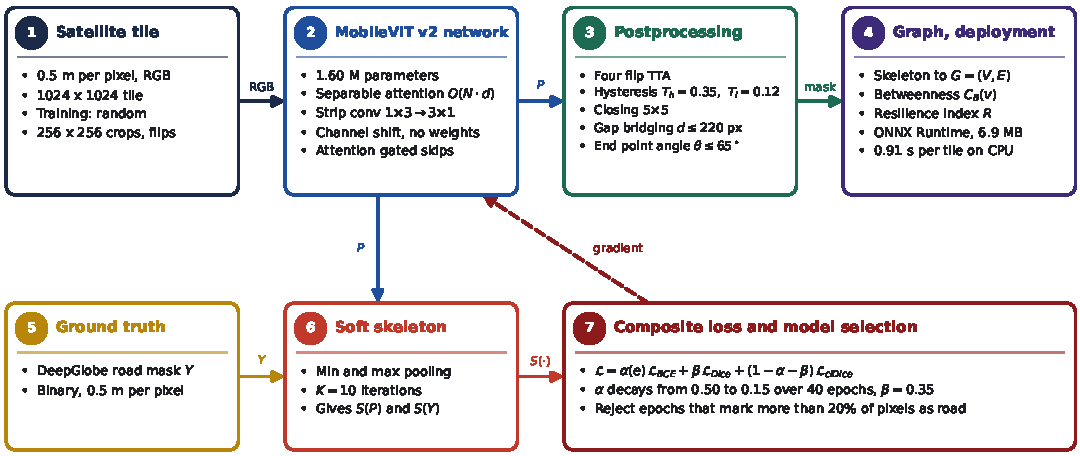
\includegraphics[width=\textwidth]{fig_system.pdf}
\caption{Overview of the system. Top row (inference): a tile passes through the network (2), the postprocessing (3), and graph construction (4). Bottom row (training): the predicted map $P$ and the true label $Y$ are reduced to centre lines (6) and compared in the loss (7), which is used to update the network.}
\label{fig:system}
\end{figure*}

\subsection{Network}

The network has the U shape common in segmentation: an encoder shrinks the image step by step while learning what it contains, and a decoder enlarges it back to full size to produce the road map (Fig.~\ref{fig:network}, Table~\ref{tab:layers}). It uses four ideas.

\begin{itemize}

\item \emph{Strip convolutions.} A normal convolution looks at a $3 \times 3$ square of pixels. Following HPLNet~\cite{cui2025hplnet}, we replace it with a $1 \times 3$ horizontal filter followed by a $3 \times 1$ vertical one. This uses 6 weights instead of 9 and suits long, thin shapes such as roads.

\item \emph{Channel shift.} Before each transformer block, a quarter of the feature channels are moved by 2 pixels up, down, left, or right. This lets each position see a little more of its surroundings at no extra cost, since nothing is learned.

\item \emph{MobileViT v2 blocks.} These transformer blocks~\cite{mehta2023separable} let every part of the tile use a summary of the whole tile, which helps to follow a road across a gap. Their cost grows only linearly with image size.

\item \emph{Attention gates.} Before encoder features are passed to the decoder, an attention gate~\cite{oktay2018attention} weights them so that road like features are kept and background such as field edges is suppressed.

\end{itemize}

\begin{figure*}[t]
\centering
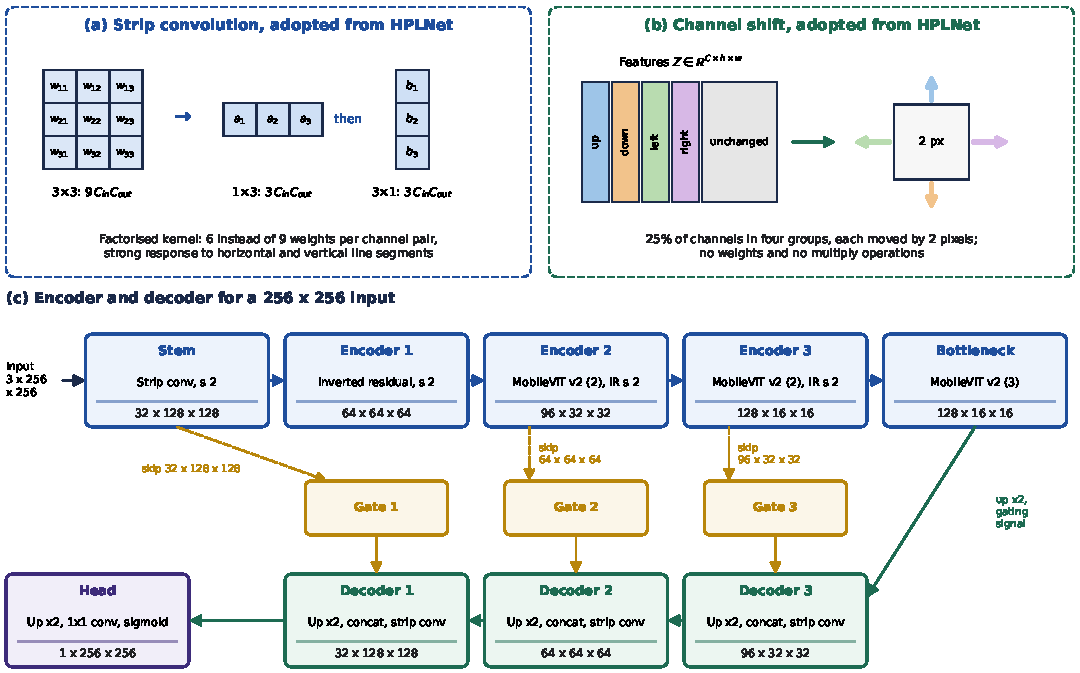
\includegraphics[width=\textwidth]{fig_network.pdf}
\caption{Network architecture. (a) Strip convolution and (b) channel shift, both taken from HPLNet~\cite{cui2025hplnet}. (c) Encoder and decoder, with the size of each output for a $256 \times 256$ input. The network accepts any input whose sides are multiples of 32.}
\label{fig:network}
\end{figure*}

\begin{table}[t]
\caption{Layer Configuration ($H$ Is the Input Height)}
\label{tab:layers}
\setlength{\tabcolsep}{3pt}
\tablebodyfont
\begin{tabular}{|p{48pt}|p{120pt}|p{50pt}|}
\hline
Stage & Operation & Output \\
\hline
Stem & Strip convolution, stride 2 & $32 \times H/2$ \\
Encoder 1 & Inverted residual, stride 2 & $64 \times H/4$ \\
Encoder 2 & MobileViT v2 block (2 layers), inverted residual, stride 2 & $96 \times H/8$ \\
Encoder 3 & MobileViT v2 block (2 layers), inverted residual, stride 2 & $128 \times H/16$ \\
Bottleneck & MobileViT v2 block (3 layers) & $128 \times H/16$ \\
Decoder & Upsample, gated skip, strip convolution & 96, 64, 32 \\
Head & Upsample, $1 \times 1$ convolution, sigmoid & $1 \times H$ \\
\hline
\end{tabular}
\end{table}

\subsection{Loss Function}

The loss tells the network how wrong its prediction is. We combine three parts:

\begin{equation}
\begin{split}
\mathcal{L} ={}& \alpha\,\mathcal{L}_{\mathrm{BCE}} + 0.35\,\mathcal{L}_{\mathrm{Dice}}\\
&+ (0.65 - \alpha)\,\mathcal{L}_{\mathrm{clDice}}.
\end{split}
\label{eq:loss}
\end{equation}

$\mathcal{L}_{\mathrm{BCE}}$ (binary cross entropy) and $\mathcal{L}_{\mathrm{Dice}}$ check each pixel; road pixels count twice in the first because roads are rare. $\mathcal{L}_{\mathrm{clDice}}$~\cite{shit2021cldice} first reduces both the prediction and the true road to centre lines one pixel wide and then measures how much of each centre line lies inside the other shape. A gap in a predicted road leaves part of the true centre line uncovered, so it raises this loss. Early in training the network cannot find roads yet, so the weight $\alpha$ starts at 0.50, favouring the pixel loss, and falls smoothly to 0.15 over the first 40 epochs, which gives the connectivity term more weight later.

\subsection{Preventing Training Collapse}

In one earlier training run the network learned to mark almost every pixel as road. This scores well on clDice, because every true road is then covered, but the map is useless. Two simple rules prevent it: the extra weight on road pixels is limited to 2, and an epoch is never saved as the best model if it marks more than 20\% of the pixels as road.

\subsection{Postprocessing}

Three steps turn the probability map into a clean road mask.

\begin{itemize}

\item \emph{Two thresholds.} Under trees the probability of a road pixel is often low. A pixel is kept if its probability is above 0.35, or above 0.12 and connected to pixels above 0.35. Faint road pieces are therefore kept only when they continue a clear road.

\item \emph{Closing.} A $5 \times 5$ morphological closing fills small holes.

\item \emph{Gap bridging.} The mask is thinned to centre lines and their loose ends are found. Two loose ends are joined by a straight line if they are at most 220 pixels apart and point roughly towards each other (within $65^{\circ}$). A loose end that remains is joined to a nearby road it points at, which completes T junctions. Ends near the tile border are ignored, because there the road simply leaves the tile.

\end{itemize}

\subsection{Road Graph Analysis}

The final mask is thinned again and converted into a graph: junctions and road ends become nodes, and the road segments between them become edges whose length is measured in pixels. For each node we compute its betweenness centrality~\cite{freeman1977betweenness}, the fraction of shortest routes between other nodes that pass through it. Nodes with high betweenness are junctions that many routes depend on. To measure how well the whole network is connected we use its global efficiency $E(G)$~\cite{latora2001efficient}, the average of one over the shortest route length between every pair of nodes; pairs with no route add zero. We then define a resilience index

\begin{equation}
R = \frac{E(\text{network without the top 10\% of nodes})}{E(\text{full network})},
\label{eq:resilience}
\end{equation}

where the removed nodes are those with the highest betweenness. A low $R$ means that losing a few key junctions, for example to a flood, would cut off part of the network.

\section{Experimental Setup}
\label{sec:setup}

\subsection{Dataset}

The DeepGlobe road extraction dataset~\cite{demir2018deepglobe} has 6,226 labelled satellite tiles of $1024 \times 1024$ pixels at 0.5~m per pixel, mostly from rural and suburban areas of Thailand, Indonesia, and India. We shuffle the tiles with a fixed random seed (42) and keep the last 10\% (623 tiles) for testing. From the remaining 5,603 tiles, 280 are set aside as a selection set for choosing the best epoch, and the other 5,323 are used for training. The 623 test tiles are therefore used only once, for the final evaluation. Our evaluation procedure rebuilds the split and checks that it matches the tile list recorded in the trained model.

\subsection{Training}

Table~\ref{tab:train} lists the settings. The model was trained from random weights, without ImageNet pretraining, on one NVIDIA Tesla T4 GPU on Kaggle, which took about 12.5 hours (4.7 min per epoch). Each step uses random $512 \times 512$ crops, so the network sees more of the surroundings of each road. Because roads run in every direction, the crops are flipped and rotated by multiples of $90^{\circ}$, and they are also slightly scaled and rotated, recoloured, and covered with synthetic tree shadows. We keep an exponential moving average (EMA) of the weights, a smoothed copy that is often more accurate than the weights at any single step. After every epoch, both the model and its EMA copy are scored on the selection set at full $1024 \times 1024$ resolution, and the best one is saved. Training is never stopped before epoch 80, and only stops early if the selection score has not improved for 40 epochs. Fig.~\ref{fig:curves} shows that the score levelled off at about 60.8\% over the last 40 epochs, so the model is not undertrained.

\begin{table}[t]
\caption{Training Configuration}
\label{tab:train}
\setlength{\tabcolsep}{3pt}
\tablebodyfont
\begin{tabular}{|p{70pt}|p{150pt}|}
\hline
Setting & Value \\
\hline
Input & Random $512 \times 512$ crops at full resolution \\
Augmentation & Flips, $90^{\circ}$ rotations, small scaling and rotation, brightness, contrast, and colour changes, synthetic tree shadows \\
Batch size & 8 \\
Optimiser & AdamW, learning rate $10^{-3}$, weight decay $10^{-4}$ \\
Schedule & 5 epoch warmup, then cosine decay to $10^{-5}$ over 160 epochs \\
Weight averaging & EMA, decay 0.999 \\
Gradient clipping & Maximum norm 1.0 \\
Precision & Mixed (FP16 and FP32) \\
Selection & 280 held out training tiles at $1024 \times 1024$; best IoU, 20\% road limit \\
Early stopping & Not before epoch 80; patience 40 (not triggered) \\
Initialisation & Random \\
Selected epoch & 158 of 160 \\
\hline
\end{tabular}
\end{table}

\begin{figure}[t]
\centering
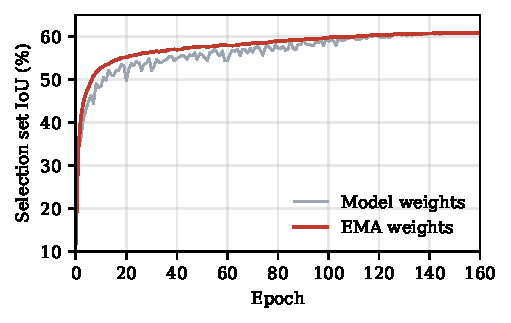
\includegraphics[width=\columnwidth]{fig_training_curves.pdf}
\caption{Selection set IoU during training for the model weights and their moving average (EMA). The score levels off over the last 40 epochs.}
\label{fig:curves}
\end{figure}

\subsection{Evaluation}

All scores are computed on the 623 test tiles at full resolution, counting pixels over the whole set. With true positives $\mathit{TP}$ (road found), false positives $\mathit{FP}$ (road predicted where there is none), and false negatives $\mathit{FN}$ (road missed),

\begin{equation}
\begin{split}
\mathrm{IoU} &= \frac{\mathit{TP}}{\mathit{TP} + \mathit{FP} + \mathit{FN}},\\
\mathrm{F1} &= \frac{2\,\mathit{TP}}{2\,\mathit{TP} + \mathit{FP} + \mathit{FN}}.
\end{split}
\label{eq:metrics}
\end{equation}

Because the labels are not perfectly aligned with the images, we also report a relaxed F1 that accepts a pixel as correct if it is within 3 pixels (1.5~m) of the true road~\cite{mnih2010roads}. The clDice score measures how much of the true centre lines is found. To study roads under trees, road pixels are split into covered and open groups using the excess green vegetation index~\cite{woebbecke1995excess} with a threshold chosen by Otsu's method~\cite{otsu1979threshold}. We compare a single pass of the network with test time augmentation (TTA), which averages the predictions for the tile and its three flipped copies, each with a fixed threshold of 0.5 or with the full postprocessing.

Speed is measured on an Intel Core i5-1035G4 laptop processor using four threads, as the average time for one $1024 \times 1024$ tile over repeated runs.

\section{Results}
\label{sec:results}

% Page wide figures are placed at the top of a later page than where they appear in the
% source, so the three wide result figures are given here, early in the section, to keep
% them ahead of the references.

\begin{figure*}[t]
\centering
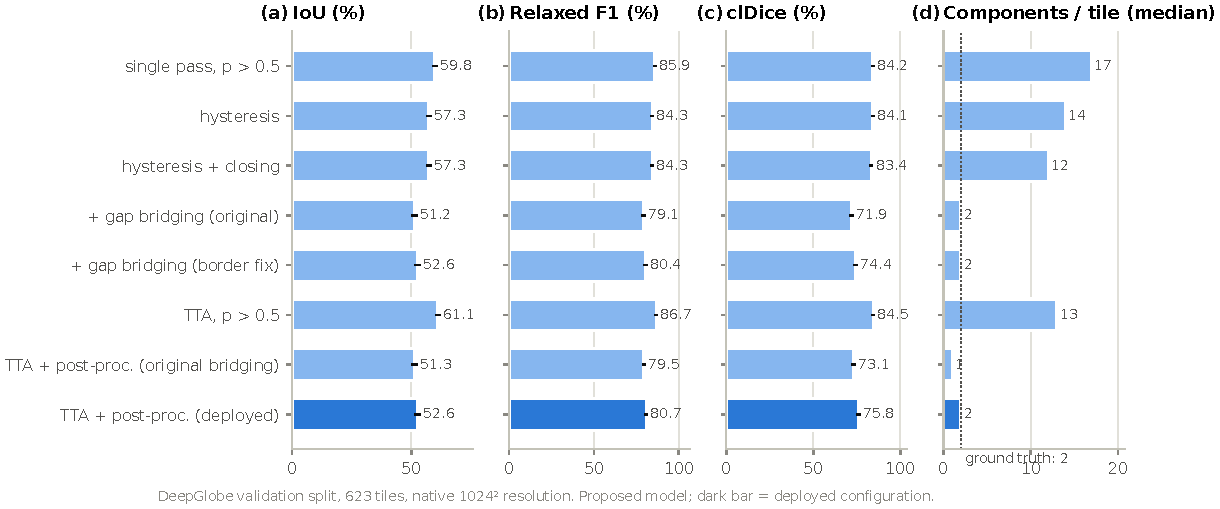
\includegraphics[width=\textwidth]{fig_inference_ablation.pdf}
\caption{Effect of each inference and postprocessing step on 623 validation tiles: (a) IoU, (b) relaxed F1, (c) clDice, and (d) median number of connected road parts per tile, with the ground truth median shown as a dotted line. The dark bar is the deployed setting. Original bridging also joins road ends at the tile border; the border fix ignores them.}
\label{fig:ablation}
\end{figure*}

\begin{figure*}[t]
\centering
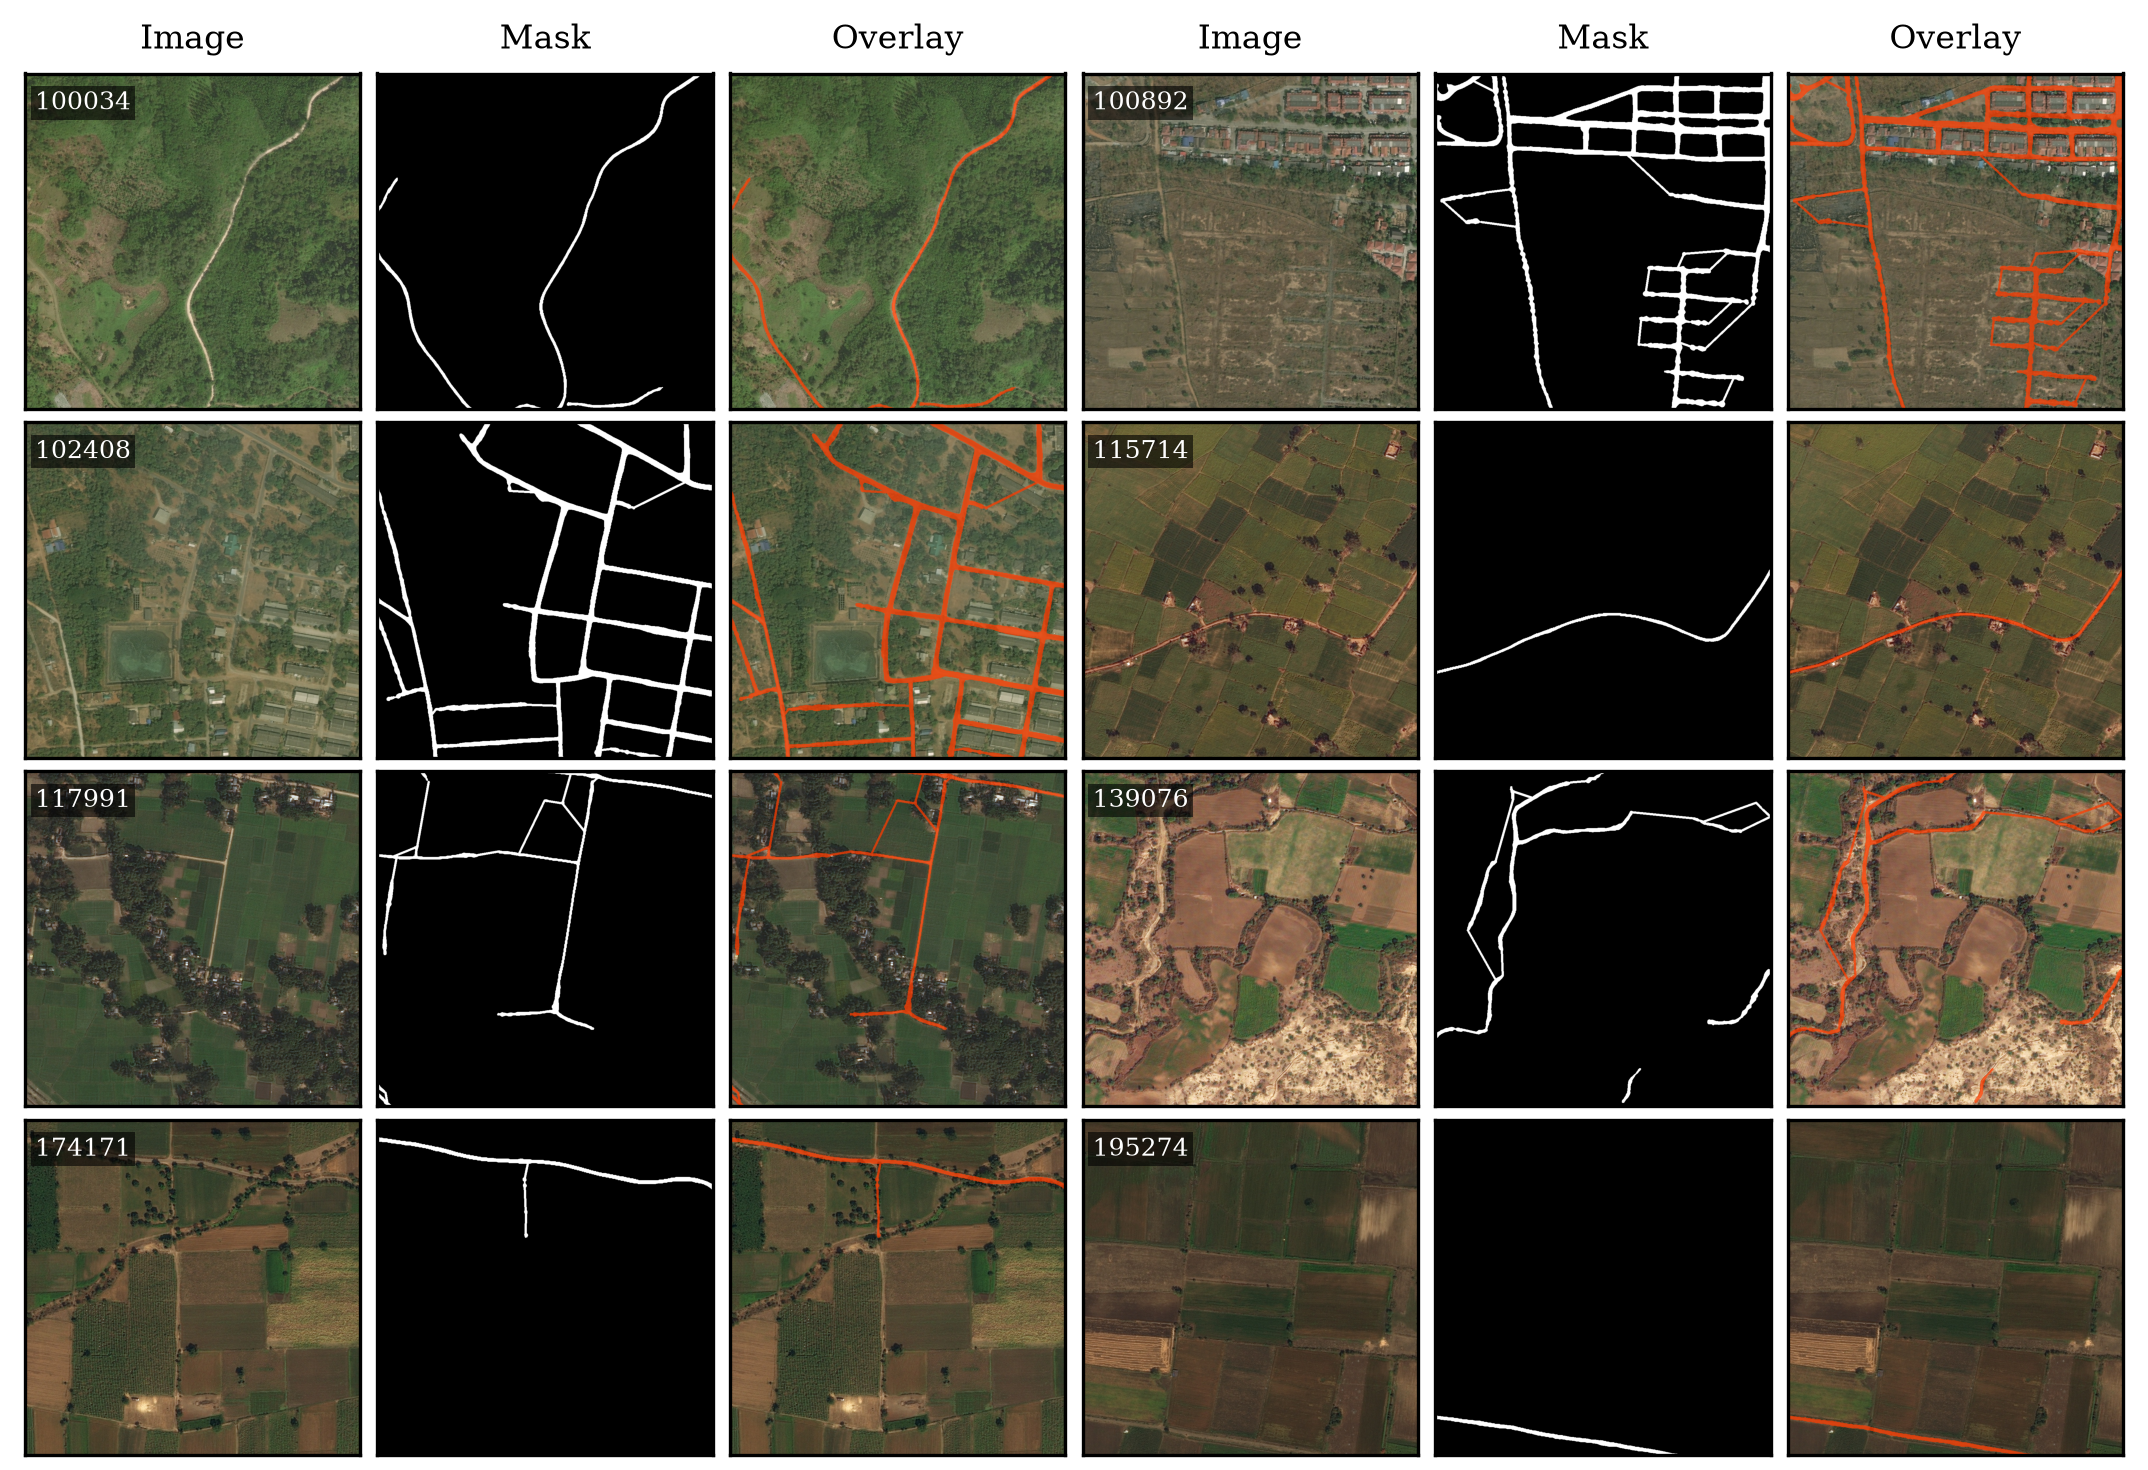
\includegraphics[width=\textwidth]{fig_predictions.png}
\caption{Output of the full pipeline (four flip TTA, hysteresis, closing, and gap bridging) on eight sample tiles. For each tile the input image, the binary mask, and the mask overlaid in orange are shown.}
\label{fig:pred}
\end{figure*}

\begin{figure*}[t]
\centering
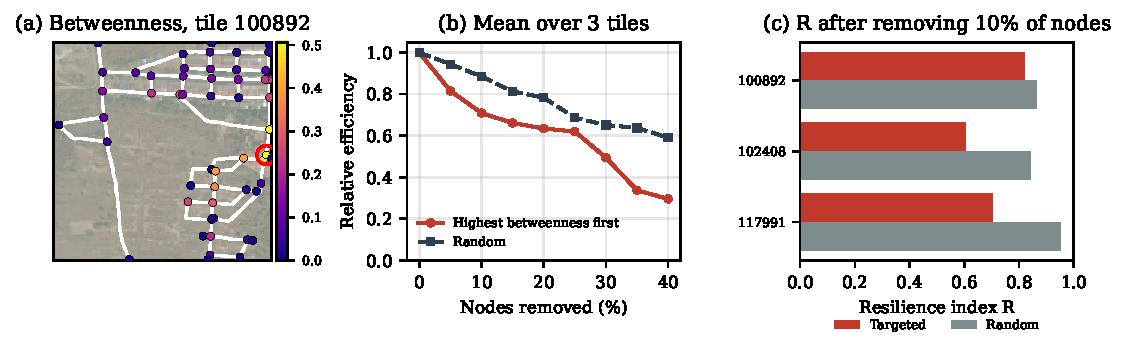
\includegraphics[width=\textwidth]{fig_graph_analysis.pdf}
\caption{Network analysis of the predicted road graphs. (a) Betweenness centrality of the nodes on tile 100892; the circled node has the highest value. (b) Relative global efficiency as nodes are removed in order of betweenness or at random (mean of 20 trials), averaged over the three tiles with at least 10 nodes. (c) Resilience index $R$ after removing 10\% of the nodes.}
\label{fig:graph}
\end{figure*}

\subsection{Model Size and Speed}

Table~\ref{tab:cost} compares the cost of the proposed network with four reference networks. All models were run with random weights in the same environment. The proposed network has 19.3 times fewer parameters and 25 times fewer operations than U-Net. With ONNX Runtime~\cite{onnxruntime} it processes a tile in 1.27 s, faster than in PyTorch. The largest difference between PyTorch and ONNX Runtime outputs over three input sizes was $1.2 \times 10^{-7}$. LR-ASPP MobileNetV3 is faster than our network in PyTorch because most of its operations are cheap depthwise convolutions, whereas our transformer blocks process high resolution feature maps.

\begin{table}[t]
\caption{Cost per $1024 \times 1024$ Tile on a Laptop Processor}
\label{tab:cost}
\setlength{\tabcolsep}{3pt}
\tablebodyfont
\begin{tabular}{|p{72pt}|r|r|r|r|}
\hline
Model & Params (M) & GFLOPs & Size (MB) & Time (s) \\
\hline
U-Net~\cite{ronneberger2015unet} & 31.04 & 1541.4 & 118.4 & 14.75$^{\mathrm{a}}$ \\
D-LinkNet34~\cite{zhou2018dlinknet} & 31.10 & 212.6 & 118.6 & 2.48 \\
DeepLabV3 MBv3~\cite{chen2017deeplab} & 11.02 & 78.6 & 42.0 & 1.00 \\
LR-ASPP MBv3~\cite{howard2019mobilenetv3} & 3.22 & 15.7 & 12.3 & 0.49 \\
Proposed (PyTorch) & 1.60 & 60.7 & 6.1 & 1.89 \\
Proposed (ONNX) & 1.60 & 60.7 & 6.2$^{\mathrm{b}}$ & 1.27$^{\mathrm{c}}$ \\
\hline
\multicolumn{5}{p{230pt}}{Sizes are FP32 weights, 1~MB $= 2^{20}$ bytes.}\\
\multicolumn{5}{p{230pt}}{$^{\mathrm{a}}$Timed as four $512 \times 512$ crops because a full tile exceeded the free memory.}\\
\multicolumn{5}{p{230pt}}{$^{\mathrm{b}}$Single ONNX file including the weights.}\\
\multicolumn{5}{p{230pt}}{$^{\mathrm{c}}$Mean of 14 runs with ONNX Runtime 1.30, measured separately from the PyTorch timings.}
\end{tabular}
\end{table}

\subsection{Accuracy}

Table~\ref{tab:acc} reports accuracy on the 623 validation tiles. The best pixel accuracy comes from TTA with a threshold of 0.5: an IoU of 61.1\% (95\% bootstrap interval 60.0\% to 62.1\%), an F1 of 75.8\%, a relaxed F1 of 86.7\%, and a clDice of 84.5\%. TTA raises the IoU of a single pass from 59.8\% to 61.1\%. With the full postprocessing, TTA gives no significant further gain (Wilcoxon signed rank test, $p = 0.48$).

\begin{table}[t]
\caption{Accuracy on 623 DeepGlobe Validation Tiles at Native Resolution (\%)}
\label{tab:acc}
\setlength{\tabcolsep}{3pt}
\tablebodyfont
\begin{tabular}{|l|c|c|c|c|c|c|c|}
\hline
Setting & P & R & F1 & IoU & Rel. F1 & clDice & Parts \\
\hline
Single, $t = 0.5$ & 71.3 & 78.8 & 74.8 & 59.8 & 85.9 & 84.2 & 17 \\
Single, hysteresis & 64.5 & 83.8 & 72.9 & 57.3 & 84.3 & 84.1 & 14 \\
Single, full & 57.8 & 85.6 & 69.0 & 52.6 & 80.4 & 74.4 & \textbf{2} \\
TTA, $t = 0.5$ & \textbf{72.7} & 79.3 & \textbf{75.8} & \textbf{61.1} & \textbf{86.7} & \textbf{84.5} & 13 \\
TTA, full & 56.6 & \textbf{88.2} & 69.0 & 52.6 & 80.7 & 75.8 & \textbf{2} \\
\hline
\multicolumn{8}{p{232pt}}{P: precision. R: recall. Rel. F1: relaxed F1 with $\rho = 3$. Parts: median number of connected road parts per tile (ground truth: 2). Full: hysteresis, closing, and gap bridging (the deployed setting with TTA).}
\end{tabular}
\end{table}

Fig.~\ref{fig:ablation} shows each postprocessing step. Hysteresis thresholding raises recall from 78.8\% to 83.8\% but lowers precision from 71.3\% to 64.5\%, so the IoU falls to 57.3\%. Gap bridging lowers the IoU further, to 52.6\%, because the bridging lines do not follow the true road width and some join unrelated segments. It does, however, reduce the median number of connected road parts per tile from 12 to 2, the same as the ground truth. The postprocessing therefore trades pixel accuracy for a connected network, which is what a road graph needs. Fig.~\ref{fig:stages} shows the stages on one tile, where bridging adds 5,674 pixels and reduces the number of parts from 9 to 2.

\begin{figure}[t]
\centering
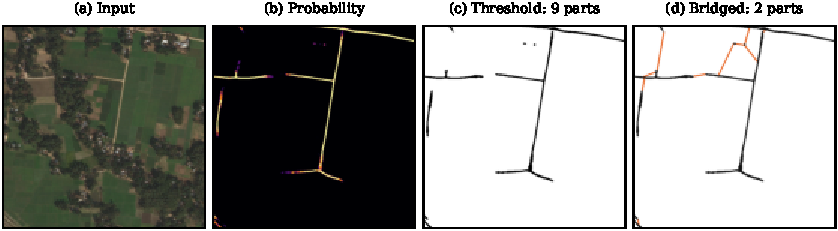
\includegraphics[width=\columnwidth]{fig_pipeline_stages.pdf}
\caption{Postprocessing on tile 117991: probability map, thresholded mask, and bridged mask.}
\label{fig:stages}
\end{figure}

\subsection{Roads Under Tree Canopy}

Table~\ref{tab:canopy} separates recall on roads under canopy from recall on open roads. With a fixed threshold, recall under canopy (60.3\% with TTA) is 20 points below recall on open road (80.3\%). Hysteresis and gap bridging raise canopy recall to 75.1\% (86.4\% relaxed) and narrow the gap to 14 points, at the cost of precision shown in Table~\ref{tab:acc}.

\begin{table}[t]
\caption{Recall on Canopy and Open Road Pixels (\%)}
\label{tab:canopy}
\setlength{\tabcolsep}{4pt}
\tablebodyfont
\begin{tabular}{|l|c|c|c|c|}
\hline
 & \multicolumn{2}{c|}{Canopy} & \multicolumn{2}{c|}{Open} \\
\cline{2-5}
Setting & Strict & Relaxed & Strict & Relaxed \\
\hline
Single, $t = 0.5$ & 59.9 & 75.9 & 79.8 & 88.3 \\
Single, hysteresis & 66.9 & 79.5 & 84.7 & 90.4 \\
Single, full & 70.3 & 83.8 & 86.4 & 92.0 \\
TTA, $t = 0.5$ & 60.3 & 76.2 & 80.3 & 88.5 \\
TTA, full & \textbf{75.1} & \textbf{86.4} & \textbf{88.9} & \textbf{93.5} \\
\hline
\multicolumn{5}{p{200pt}}{Canopy pixels: excess green index above the Otsu threshold (0.119).}
\end{tabular}
\end{table}

\subsection{Effect of the Training Recipe}

Our first full resolution run (v3) used the same network and loss but a shorter recipe: 50 epochs, $256 \times 256$ crops, only flips and colour changes, no weight averaging, and the tree shadow augmentation inactive because of a software version problem. Its best validation score was reached at the last epoch, a sign that it was still improving. Table~\ref{tab:recipe} compares it with the final recipe on the same 623 test tiles. The final model is better on every measure; its IoU is higher on 90\% of the tiles, with a mean gain of 8.8 points per tile (Wilcoxon signed rank test, $p < 10^{-80}$). Recall under canopy rises the most, from 43.1\% to 60.3\%, which suggests that the tree shadow augmentation and the larger crops help most where roads are hidden. The v3 epoch was chosen on the test tiles themselves, which can only favour v3, so the true gain is if anything larger.

\begin{table}[t]
\caption{Effect of the Training Recipe on the 623 Test Tiles (\%)}
\label{tab:recipe}
\setlength{\tabcolsep}{3pt}
\tablebodyfont
\begin{tabular}{|l|c|c|c|c|c|}
\hline
Model, inference & IoU & F1 & Rel. F1 & clDice & Canopy R \\
\hline
v3, TTA, $t = 0.5$ & 52.7 & 69.0 & 79.9 & 76.8 & 43.1 \\
Final, TTA, $t = 0.5$ & \textbf{61.1} & \textbf{75.8} & \textbf{86.7} & \textbf{84.5} & 60.3 \\
v3, TTA, full & 43.4 & 60.5 & 72.5 & 67.1 & 63.0 \\
Final, TTA, full & 52.6 & 69.0 & 80.7 & 75.8 & \textbf{75.1} \\
\hline
\multicolumn{6}{p{215pt}}{v3: 50 epochs, $256 \times 256$ crops, flips and colour only. Final: Table~\ref{tab:train}. Canopy R: recall on road pixels under tree cover.}
\end{tabular}
\end{table}

Two earlier problems also shaped the protocol. One run collapsed at epoch 46 and marked 80.9\% of the pixels of four sample tiles as road; the 20\% gate of Section~\ref{sec:method} now rejects such epochs. Earlier runs also validated on tiles resized to $256 \times 256$ pixels, which made roads four times thinner than in training and misled the choice of epoch; all later runs validate at full resolution.

\subsection{Qualitative Results}

Fig.~\ref{fig:pred} shows the output of the full pipeline on eight rural sample tiles. Roads through forest, farmland, and villages are recovered as continuous lines. Some thin straight segments, for example on tiles 100892 and 139076, are added by gap bridging and do not follow a visible road. On tile 195274, which has only faint field tracks, the model finds the track along the lower edge but misses the others, an example of the lower recall on narrow, low contrast roads.

\subsection{Road Network Analysis}

Fig.~\ref{fig:graph} applies the analysis of Section~\ref{sec:method} to the predicted graphs of the sample tiles. Three tiles, 100892, 102408, and 117991, produce a connected network of at least 10 nodes; the others contain one or two roads, for which the analysis is not meaningful. The largest graph, on tile 100892, has 55 nodes and 72 edges. Removing the 10\% of nodes with the highest betweenness lowers the mean relative efficiency to 0.71, against 0.89 for random removal; after removing 40\% of the nodes it falls to 0.30, against 0.59. Removing the most central junctions therefore always does more damage than removing junctions at random. Tile 102408 has the lowest resilience index ($R = 0.61$). These graphs are built from predictions, not from ground truth, so the analysis shows how the extracted network can be used for planning rather than measuring accuracy.


\section{Discussion and Limitations}
\label{sec:discussion}

The network has fewer than two million parameters and processes a tile in about 1.3 s on a laptop processor without a graphics card. Its relaxed F1 of 86.7\% and clDice of 84.5\% show that most road centrelines are recovered. Several limitations remain.

\begin{itemize}

\item \emph{No baselines on the same split.} The reference networks in Table~\ref{tab:cost} were compared on cost only. Accuracy figures published for DeepGlobe use different splits and cannot be compared directly with Table~\ref{tab:acc}. Training the reference networks on our split is required for a fair accuracy comparison.

\item \emph{No pretraining.} The encoder was trained from random weights because its custom layers do not match standard ImageNet weights. Training converged (Fig.~\ref{fig:curves}), so further gains are more likely to come from pretraining or more data than from more epochs.

\item \emph{Heuristic bridging.} The bridging rules use fixed distances in pixels and depend on the ground sampling distance. They can also create false links.

\item \emph{Single dataset.} DeepGlobe covers rural areas but not specifically PMGSY roads. Validation on Indian rural imagery is future work.

\end{itemize}

\section{Conclusion}
\label{sec:conclusion}

We presented a road extraction network with 1.60 million parameters that combines MobileViT v2 attention, attention gates, and road shaped convolutions, trained with a connectivity aware loss and followed by geometric gap bridging. At native resolution on 623 held out DeepGlobe tiles it reaches an IoU of 61.1\%, a relaxed F1 of 86.7\%, and a clDice of 84.5\%, and it runs in 1.27 s per tile on a laptop processor without a deep learning framework. Recall on roads under tree canopy remains 20 points below recall on open roads; the postprocessing narrows this gap to 14 points and yields a connected network with as few parts as the ground truth. A longer training recipe with stronger augmentation gave the largest single improvement, 8.4 points of IoU. Future work will pretrain the encoder, train the reference networks on the same split, replace the heuristic bridging with a learned connection model, and evaluate on Indian rural imagery.

\section*{Data Availability}

The DeepGlobe road extraction dataset is publicly available from the DeepGlobe 2018 challenge~\cite{demir2018deepglobe}. The eight sample tiles in Fig.~\ref{fig:pred} and the measurement files used in this paper are included with the supplementary material. The identifiers of the 623 validation tiles are provided with the supplementary material.

\section*{Conflict of Interest}

The authors declare that they have no known competing financial interests or personal relationships that could have appeared to influence the work reported in this paper.

\section*{Acknowledgment}

The authors thank the IEEE Computer Society Bangalore Chapter for the internship and mentorship program, and the organisers of the DeepGlobe 2018 challenge for releasing the dataset.

\begin{thebibliography}{00}

\bibitem{pmgsy}
Ministry of Rural Development, Government of India,
``Pradhan Mantri Gram Sadak Yojana.''

\bibitem{ronneberger2015unet}
O. Ronneberger, P. Fischer, and T. Brox,
``U-Net: Convolutional networks for biomedical image segmentation,''
in \emph{Proc. Int. Conf. Med. Image Comput. Comput.-Assist. Intervent. (MICCAI)},
Munich, Germany, 2015, pp. 234--241.

\bibitem{zhou2018dlinknet}
L. Zhou, C. Zhang, and M. Wu,
``D-LinkNet: LinkNet with pretrained encoder and dilated convolution for high resolution satellite imagery road extraction,''
in \emph{Proc. IEEE/CVF Conf. Comput. Vis. Pattern Recognit. Workshops (CVPRW)},
Salt Lake City, UT, USA, 2018, pp. 182--186.

\bibitem{mehta2023separable}
S. Mehta and M. Rastegari,
``Separable self-attention for mobile vision transformers,''
\emph{Trans. Mach. Learn. Res.}, 2023.

\bibitem{oktay2018attention}
O. Oktay \emph{et al.},
``Attention U-Net: Learning where to look for the pancreas,''
in \emph{Proc. Med. Imag. Deep Learn. (MIDL)},
Amsterdam, The Netherlands, 2018.

\bibitem{cui2025hplnet}
S. Cui, Q. Feng, L. Ji, X. Liu, and B. Guo,
``HPLNet: A hierarchical perception lightweight network for road extraction,''
\emph{Front. Remote Sens.}, vol. 6, Sep. 2025, Art. no. 1668978,
doi: 10.3389/frsen.2025.1668978.

\bibitem{shit2021cldice}
S. Shit \emph{et al.},
``clDice: A novel topology-preserving loss function for tubular structure segmentation,''
in \emph{Proc. IEEE/CVF Conf. Comput. Vis. Pattern Recognit. (CVPR)},
2021, pp. 16560--16569.

\bibitem{chen2017deeplab}
L.-C. Chen, G. Papandreou, F. Schroff, and H. Adam,
``Rethinking atrous convolution for semantic image segmentation,''
2017, \emph{arXiv:1706.05587}.

\bibitem{demir2018deepglobe}
I. Demir \emph{et al.},
``DeepGlobe 2018: A challenge to parse the Earth through satellite images,''
in \emph{Proc. IEEE/CVF Conf. Comput. Vis. Pattern Recognit. Workshops (CVPRW)},
Salt Lake City, UT, USA, 2018, pp. 172--181.

\bibitem{sandler2018mobilenetv2}
M. Sandler, A. Howard, M. Zhu, A. Zhmoginov, and L.-C. Chen,
``MobileNetV2: Inverted residuals and linear bottlenecks,''
in \emph{Proc. IEEE/CVF Conf. Comput. Vis. Pattern Recognit. (CVPR)},
2018, pp. 4510--4520.

\bibitem{howard2019mobilenetv3}
A. Howard \emph{et al.},
``Searching for MobileNetV3,''
in \emph{Proc. IEEE/CVF Int. Conf. Comput. Vis. (ICCV)},
Seoul, South Korea, 2019, pp. 1314--1324.

\bibitem{mehta2022mobilevit}
S. Mehta and M. Rastegari,
``MobileViT: Light-weight, general-purpose, and mobile-friendly vision transformer,''
in \emph{Proc. Int. Conf. Learn. Represent. (ICLR)},
2022.

\bibitem{bastani2018roadtracer}
F. Bastani \emph{et al.},
``RoadTracer: Automatic extraction of road networks from aerial images,''
in \emph{Proc. IEEE/CVF Conf. Comput. Vis. Pattern Recognit. (CVPR)},
Salt Lake City, UT, USA, 2018, pp. 4720--4728.

\bibitem{he2020sat2graph}
S. He \emph{et al.},
``Sat2Graph: Road graph extraction through graph-tensor encoding,''
in \emph{Proc. Eur. Conf. Comput. Vis. (ECCV)},
2020, pp. 51--67.

\bibitem{vanetten2018spacenet}
A. Van Etten, D. Lindenbaum, and T. M. Bacastow,
``SpaceNet: A remote sensing dataset and challenge series,''
2018, \emph{arXiv:1807.01232}.

\bibitem{mnih2010roads}
V. Mnih and G. E. Hinton,
``Learning to detect roads in high-resolution aerial images,''
in \emph{Proc. Eur. Conf. Comput. Vis. (ECCV)},
Heraklion, Greece, 2010, pp. 210--223.

\bibitem{woebbecke1995excess}
D. M. Woebbecke, G. E. Meyer, K. Von Bargen, and D. A. Mortensen,
``Color indices for weed identification under various soil, residue, and lighting conditions,''
\emph{Trans. ASAE}, vol. 38, no. 1, pp. 259--269, 1995.

\bibitem{otsu1979threshold}
N. Otsu,
``A threshold selection method from gray-level histograms,''
\emph{IEEE Trans. Syst., Man, Cybern.}, vol. SMC-9, no. 1, pp. 62--66,
Jan. 1979.

\bibitem{freeman1977betweenness}
L. C. Freeman,
``A set of measures of centrality based on betweenness,''
\emph{Sociometry}, vol. 40, no. 1, pp. 35--41,
Mar. 1977.

\bibitem{latora2001efficient}
V. Latora and M. Marchiori,
``Efficient behavior of small-world networks,''
\emph{Phys. Rev. Lett.}, vol. 87, no. 19, Oct. 2001,
Art. no. 198701.

\bibitem{onnxruntime}
ONNX Runtime developers,
``ONNX Runtime.''

\end{thebibliography}

\begin{IEEEbiography}{Dilraj Singh}
is currently pursuing the B.E. degree in computer science and engineering
(artificial intelligence and machine learning) at R. V. College of Engineering,
Bengaluru, India. [Research interests.]
\end{IEEEbiography}

\begin{IEEEbiography}{Arya Wadhwa}
is currently pursuing the B.E. degree in computer science and engineering
(artificial intelligence and machine learning) at R. V. College of Engineering,
Bengaluru, India. [Research interests.]
\end{IEEEbiography}

\EOD

\end{document}
